%%%%%%%%%%%%%%%%%%%%%%%%%%%%%%%%%%%%%%%%%%%%%%%%%%%%%%%%%%%%%%%%%%% 
%                                                                 %
%                       LITERATUURSTUDIE                          %
%                                                                 %
%%%%%%%%%%%%%%%%%%%%%%%%%%%%%%%%%%%%%%%%%%%%%%%%%%%%%%%%%%%%%%%%%%% 

\chapter{Literatuurstudie}

In dit hoofdstuk gaan we kijken wat er in de literatuur te vinden is over een aantal verschillende topics.
Het eerste topic is de combinatie van indoor navigatie en visie (~\ref{sec:nav_visie}).
In een tweede hoofdstuk gaan we kijken naar de verschillende objectdetectie technieken (\ref{sec:object_det}).
Vervolgens zullen we kijken naar object tracking, of het volgen van objecten tussen frames (\ref{sec:object_det}).
Het laatste onderwerp dat we zullen bekijken is image segmentation (\ref{sec:image_segmentation}).

    \section{Indoor navigatie \& visie} \label{sec:nav_visie}
        Op visie gebaseerde navigatie is een onderwerp dat zeer vaak onderzocht wordt. Oudere onderzoeken zoals~\cite{Tomono2000} maken gebruik van een robot met een \gls{rgb} camera die zonder kaart informatie navigeert.
        De enige informatie die gegeven wordt is een eenvoudige object beschrijving van de gang en een beschrijving van een deur met een deurnummer ernaast.
        Met enkel een deurnummer als doel vertrekt de robot door de gang, en houdt zichzelf parallel met de muren door gebruik te maken van andere sensoren.
        Eens er een deur in beeld komt, worden er features zoals randen herkend in het beeld.
        Nadat hun algoritme de deuren herkent kan er via \gls{ocr} op het deurnummer worden nagegaan of het doel bereikt is.
        Dit is uiteraard een zeer eenvoudige techniek omdat de robot geen begrip heeft van de omgeving, en moeilijk plaatsen t.o.v elkaar kan onderscheiden.
        Bovendien zijn in onze ziekenhuisgangbeelden weinig deuren zichtbaar waar we de deurnummers niet kunnen gebruiken als feature.

%        Nieuwere technieken zoals~\cite{Henry10rgb-dmapping} maken gebruik van RGB-D camera's zoals bijvoorbeeld een kinect waardoor ze ook over diepte-informatie beschikken.
%        Die diepte info kan dan gebruikt worden om heel de omgeving in 3d te mappen en op basis van de effectief gemeten positie te navigeren.
%        Een andere manier om een 3d representatie van de omgeving te verkrijgen zoals~\cite{schmid2013} is gebruik te maken van stereovisie.
%        Hierbij wordt de informatie van 2 \gls{rgb} camera's die op een vaste afstand van elkaar staan gecombineerd om diepte informatie te verzamelen.
%        In dit onderzoek gaan we ons echter beperken tot \'{e}\'{e}n enkele \gls{rgb} camera.

        Goedem\'{e} et al~\cite{goedeme2007omnidirectional} gebruikte een topologische kaart, wat ook semantische informatie is.
        De informatie op onze kaart is echter verschillend.
        Bovendien maakten deze auteurs gebruik van omnidirectionele camera's zodat de detectie van het vluchtpunt vermeden werd.
        
        
    \section{Object detectie}\label{sec:object_det}

        Een belangrijk aspect van dit onderzoek is het detecteren van individuele objecten in het beeld van \'{e}\'{e}n enkele \gls{rgb} camera.
        De te detecteren objecten zijn op voorhand vastgelegd, en zijn afhankelijk van de ruimte waarin de robot zich bevindt.

        In de logistieke gangen van een ziekenhuis zijn er heel wat objecten die we kunnen detecteren, een kleine selectie van deze objecten zijn:

        \begin{itemize}
            \item Pictogrammen;
            \item Brandblussers;
            \item Deurklinken.
        \end{itemize}

        Voor deze objecten gaan we kijken naar detectietechnieken uit de traditionele beeldverwerking, en naar deep-learning gebaseerde technieken.


        \subsection{Traditionele beeldverwerking} \label{sec:trad_obj_det}
            In openbare gebouwen zijn er heel wat pictogrammen te vinden zoals bijvoorbeeld nooduitgang, hoogspanning en brandblusser. Deze pictogrammen hebben steeds een specifieke vorm, kleur en symbool.
            De literatuur over pictogramdetectie is schaars. De techniek die voorgesteld wordt door~\cite{swathika2016} gebruikt een zeer eenvoudige edge detectie met \gls{ocr} om eventuele letters op pictogrammen te lezen, dit is echter minder relevant omdat niet op elk pictogram tekst aanwezig is. Pictogrammen kunnen echter wel vergeleken worden met verkeersborden die bijna dezelfde kenmerken hebben.
            De aanpak van~\cite{Fang2003} is om 2 soorten features in een beeld te onderscheiden. Enerzijds detecteren ze vormen op basis van kleurranden en anderzijds wordt de
            afbeelding omgezet naar \gls{hsi} waaruit enkel de hue gebruikt wordt. De hue is de belangrijkste component voor het onderscheiden van kleuren omdat er zo geen rekening wordt gehouden
            met de hoeveelheid licht en schaduwen.
            Een recenter onderzoek~\cite{Zabihi2017} bouwt voort op deze technieken, maar hier berekenen ze de \gls{hog} features van het beeld.
            Vervolgens wordt er gebruik gemaakt van een \gls{svm} om te bepalen waar er zich een match bevindt.

            Een \gls{svm} is volgens~\cite{fradkin2006support} een binaire classificatie techniek die gebruikt kan worden om na te kijken bij welk klasse een feature het dichtst aanleunt.
            De scheiding tussen de 2 klassen wordt voorgesteld door een hypervlak dat bepaald wordt door middel van voorbeelden in de trainingsfase.
            Een feature wordt geclassificeerd door te kijken aan welke kant van het hypervlak hij het beste past.

            De vorm en kleur features kunnen dan gecombineerd worden om de positie van een mogelijke match te vinden. Eens er een mogelijke boundig box rond de mogelijke match gevonden is,
            kan er geprobeerd worden een template te matchen om het effectieve pictogram te achterhalen. Het grootste probleem bij de techniek van~\cite{Fang2003} is
            dat hun gebruikte template matching techniek niet robuust is tegen schaalinvariantie.
            Bij~\cite{Zabihi2017} maken ze voor de herkenningsfase gebruik van \gls{sift}\cite{Lowe1999} features en kleur informatie.
            Hierdoor is het probleem van schaalinvariantie grotendeels opgelost.
            Hierbij worden de \gls{sift} features van de kandidaat matches en de templates vergeleken, en wordt er een gemiddelde genomen van de verschillen tussen hue, saturation en value.
            Door middel van \gls{ransac} en een treshold wordt er bepaald welke matches gebruikt worden. Deze techniek zou gebruikt kunnen worden voor het detecteren van pictogrammen.

        
        \subsection{Convolutional neural nework} \label{sec:yolo}
            De laatste jaren in het domein van beeldverwerking wordt er steeds meer gegrepen naar deep learning technieken.
            Dit komt omdat de rekenkracht van computers steeds beter en beter wordt, en de resultaten die bekomen worden met neurale netwerken de traditionele manieren overtreffen op verschillende vlakken.
            Een deep learning techniek die veel gebruikt wordt in de beeldverwerking is een \gls{cnn}.

            Een \gls{cnn} is een supervised deep learning techniek die gebruikt kan worden om verschillende beeldverwerkende taken uit te voeren.
            Als een traditioneel neuraal netwerk gebruikt zou worden voor een afbeelding van 448 bij 448 pixels, zou er bij elke inwendige laag van 40 neuronen ongeveer 8 miljoen variabele gewichten aanwezig moeten zijn,
            dit zou leiden tot een veel te complex netwerk.
            Daarom wordt er gebruikgemaakt van een \gls{cnn}, dit is eigenlijk een neuraal netwerk waarbij niet alle neuronen met elkaar verbonden zijn.~\cite{lecun1990handwritten}

            Een \gls{cnn} kan bestaan uit meerdere lagen die meestal een combinatie zijn van 'convolutional-layers' en 'fully connected-layers'.
            Elk van deze lagen bevat een aantal neuronen met elk een eigen set van gewichten.
            Het doel van een \gls{cnn} is om de gewichten zodanig bij te stellen dat data gegeven aan de eerste laag (de input laag) een resultaat zoals een classificatie met een nauwkeurigheid geeft aan de laatste laag (de output/classificatie laag).
            Deze laatste laag kan men de classificatielaag noemen, en geeft een representatie van wat het netwerk denkt dat er aan de input staat.
            In figuur~\ref{fig:yolo_cnn} is een voorbeeld zichtbaar van een \gls{cnn} met de verschillende soorten lagen.

            \begin{figure}[!htb]
                \centering
                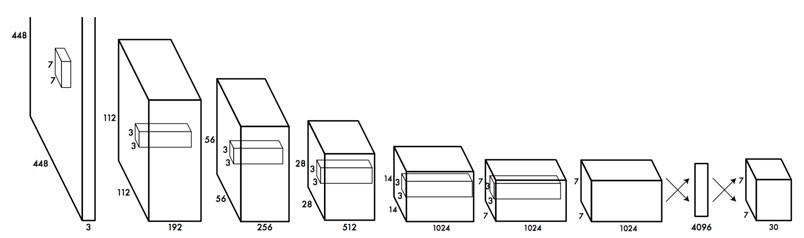
\includegraphics[width=0.75\linewidth]{literatuurstudie/yolo_cnn.jpeg}
                \caption{De lagen van een CNN volgens het YOLO~\cite{Redmon_2016} detection system.}
                \label{fig:yolo_cnn}
            \end{figure}

            Een 'convolutional-layer' of convolutie-laag is een laag die een convolutie operatie uitvoert op zijn input.
            Dit wil zeggen dat de input verdeeld wordt in regio's van bijvoorbeeld 7x7 pixels, deze 49 pixels zijn verbonden met 1 neuron in de volgende inwendige laag.
            Als dit 7x7 masker wordt opgeschoven met 1 pixel, verkrijgen we de input voor aan andere neuron in de volgende laag.
            Dit proces kan gebeuren in meerdere dimensies tegelijkertijd, op dat moment spreekt men van een tensormasker.
            Een voorbeeld van een convolutie in meerdere dimensies tegelijkertijd is een \gls{rgb} afbeelding die in een keer door het netwerk gaat, waarbij de dimensies de rode, groene en blauwe pixels van het beeld zijn.

            De verschillende inwendige lagen van een \gls{cnn} zullen na training op zoek gaan naar features. Deze features kunnen eenvoudig zijn zoals randen en lijnen, maar kunnen ook complexer zijn specifiek voor de getrainde data.
            Elke laag genereert dus een soort featuremap, die gebruikt wordt als input voor de volgende laag van het netwerk.

            Om uiteindelijk een classificatie te verkrijgen moet er een dimensievermindering doorgevoerd worden, dit wordt gedaan door 'pooling layers' aan het netwerk toe te voegen na elke convolutie laag.
            Dit heeft ook als effect dat de featuremaps vereenvoudigd worden, en het aantal gewichten beperkt blijft.

            Een CNN kan pas gebruikt worden nadat het getraind is. Voor de training van een netwerk zijn er 2 dingen noodzakelijk: voorbeeld data en per voorbeeld de verwachte output (label).
            Bij het trainingsproces wordt alle inputdata aangelegd, en wordt er gekeken wat het netwerk aan zijn output heeft.
            De loss functie is een maat van hoe goed een netwerk een voorspelling kan doen van de input data, met andere woorden een vergelijking tussen de input en de output.
            Trainen van een netwerk is het optimaliseren van de gewichten bij de neuronen in elke laag van het netwerk, bij een optimaal resultaat is de loss functie minimaal.
            Dit is een complex probleem dat enkel kan lukken indien er genoeg trainingsdata ter beschikking is.
            Trainen kan gedaan worden d.m.v 'backprogagation'\cite{lecun2012efficient}.

            De kost van een netwerk is afhankelijk van alle gewichten die zich in het netwerk bevinden.
            Om de kost te minimaliseren dienen al deze gewichten zo goed mogelijk afgestemd te worden op basis van de trainingsvoorbeelden.
            Een neuraal netwerk propageert data van de input door al zijn parameters tot aan de laatste laag waar de beslissing genomen wordt.
            Op dit moment kan de eindbeslissing vergeleken worden met het trainingslabel en achteruit gepropageerd worden (backpropagation) met informatie over de gemaakte fout.
            Zo kan het netwerk gecorrigeerd worden 1 gewicht per keer.
            Doordat de gewichten zich in lagen bevinden, en dus onderling afhankelijk zijn, moet de kettingregel toegepast worden om de waarden te corrigeren.
            Een meer gedetailleerde uitleg over de wiskunde achter backpropagation is beschreven door~\cite{nielsenneural}.

            Een belangrijke laag in een \gls{cnn} is de \gls{relu}~\cite{NIPS2012_4824}.
            Deze laag voegt een niet lineaire functie toe tussen de convolutielagen, dit is nodig omdat de convolutie een lineaire operatie is, en een eigenschap van lineaire operators laat toe om deze te combineren tot 1 operator.
            Dit zou willen zeggen dat alle convoluties in een netwerk gereduceerd kunnen worden tot 1 laag, en dus het voordeel van meerdere lagen wegnemen.
            Het toevoegen van een \gls{relu} laag tussen elke convolutielaag voorkomt dit probleem.

            Een voorbeeld van een CNN is het '\gls{yolo} detection system'~\cite{Redmon_2016}. Het \gls{yolo} netwerk is opgebouwd uit 24 convolutielagen en 2 'fully connected' lagen.
            Dit netwerk heeft een uitgebreide training gehad op de ImageNet dataset\footnote{http://www.image-net.org} en kan gebruikt worden om objectdetectie en -classificatie te doen door \'{e}\'{e}n keer de input afbeelding door het netwerk te laten gaan.
            Door middel van een hertraining kan deze detector leren om alle objecten te detecteren en te classificeren en dus een mogelijke detector zijn voor onze toepassing.

            Zoals~\cite{Llopart2017} voorstelt is het niet moeilijk om het '\gls{yolo} detection system' een hertraining te geven om deuren te herkennen. Zo kan dit ook toegevoegd worden aan de lijst met te detecteren kenmerken. 


    \section{Object tracking} \label{sec:obj_tracking}
        Object tracking of het volgen van objecten heeft als doel het bepalen van de positie van hetzelfde object over meerdere frames heen. In het geval van dit onderzoek kan het een indicatie geven van relatieve posities t.o.v. objecten die zich in de gangen bevinden.
        Een grote moeilijkheid bij het volgen van objecten die stilstaan t.o.v. de bewegende camera is dat ze veranderen in grootte, ori\"{e}ntatie en perspectief.
        \cite{Zhou2009} stelt voor om gebruik te maken van \gls{sift} voor het volgen van objecten. Ze zoeken een \gls{roi} op het eerste frame waarop ze een kleurhistogram en \gls{sift} features berekenen.
        Op het volgende frame worden dezelfde bewerkingen uitgevoerd in een regio die net iets groter is dan de originele \gls{roi}. Een overeenkomstregio wordt dan berekend door middel van een \gls{em} algoritme.
        Volgens~\cite{Baheti2016} is het beter om gebruik te maken van het KLT feature algoritme~\cite{tomasi1991detection}. Hiermee wordt er een transformatie berekent waardoor de \gls{roi} tussen de 2 frames gelijkaardig wordt. De initi\"{e}le transformatieparameters worden berekend via \gls{ransac}.

        \cite{Ning2017} heeft een nieuwe techniek ontwikkeld om object tracking te combineren met object detectie \gls{cnn}. Ze hebben een uitbreiding gemaakt op het \gls{yolo} detection system genaamd \gls{rolo}.
        De uitbreiding bevat een extra \gls{lstm} geplaatst achter de detectie fase van het originele netwerk. Een \gls{lstm} is een neuraal netwerk geoptimaliseerd voor het maken van beslissingen op tijdsgebaseerde data.
        De data die aan het extra netwerk gegeven wordt is een van de tussenresultaten van het \gls{yolo} netwerk.
        Het systeem blijkt zeer goed te werken voor het volgen van objecten zelfs bij occlusies in \'{e}\'{e}n van de beelden.
        Momenteel is deze techniek niet gebruikt in onze implementatie, maar zou in de toekomst wel kunnen helpen om te nauwkeurigheid te verhogen.

    \section{Image segmentation}\label{sec:image_segmentation}
        Het correct segmenteren van de beelden zal een belangrijke rol spelen in dit onderzoek.
        Het segmenteren van een beeld wil zeggen dat we pixels gaan groeperen in een aantal klassen.
        Niet in elk beeld van ziekenhuisgangen zal er een distinctief object aanwezig zijn om te detecteren. Daarom is het belangrijk om de vloer van
        de muren te kunnen onderscheiden. Een eenvoudige aanpak zou kunnen zijn om via K-means een verdeling van een beeld te doen en met regressie de regio's te labelen.
        Volgens~\cite{zhangwall} werkt de K-means aanpak met een op textuur en kleur gebaseerde aanpak redelijk goed, maar wordt steeds de muur verbonden met het plafond omwille van kleur en textuurgelijkenissen.
        Hun regressie gebaseerde labeling techniek blijkt dus een slechte oplossing.
        Een mogelijke verbetering zou kunnen zijn om de kennis toe te voegen dat een plafond zich steeds boven de vloer bevindt, hierbij zou de blob in 2 delen gesplitst kunnen worden om de vloer te verkrijgen.
        Verder zoals~\cite{Li2010} aangeeft zijn reflecties en overbelichting eigenschappen van indoor omgevingen die het moeilijk kunnen maken om
        een correcte segmentatie te doen.
        \cite{Li2010} stelt een techniek voor die begint met het detecteren van verticale en horizontale lijn segmenten. Dit doen ze door eerst een Canny edge detector\cite{Canny} toe te passen en vervolgens een line fitting.
        Een zelf geleerde \gls{svm} classifier verdeeldt alle lijnsegmenten in twee categorie\"{e}n: horizontaal en verticaal. De vluchtlijnen van de gang worden hierbij onderverdeeld in de horizontale categorie.
        Alle lijnstukken krijgen een score via een reeks van operaties waarna enkel de beste lijnen bijgehouden worden. Op basis van de kleur van de vlakken tussen de lijnstukken kan een segmentatie gemaakt worden.
        Dit geeft een resultaat waarbij de vloer meestal een mooi homogeen geheel is, maar de muren in meerdere vlakken gesegmenteerd worden door eventuele kleurverschillen en objecten aan de muur.
        
        Een andere manier om de vloer te segmenteren is voorgesteld in~\cite{Rodriguez-Telles2013}. Zij doen een superpixel segmentatie volgens het SLIC algoritme~\cite{slic}, vervolgens bekijken ze de randen van de superpixels.
        Na observaties blijkt dat de randen van superpixels onregelmatig worden bij objectovergangen. Door het aanduiden van een paar vloerpixels kan hun algoritme superpixels aanduiden die tot de vloer behoren.
        Deze aanpak geeft een goede schatting van vrije ruimte op de vloer, maar is minder bruikbaar voor segmentatie van muren.

        Een meer recente technologie om afbeeldingen te segmenteren is gebruik te maken van een \gls{cnn}. Het netwerk voor segmentatie is verschillend van een traditioneel \gls{cnn} voor bijvoorbeeld object detectie.
        Een voorbeeld van een segmentatienetwerk is te zien in figuur~\ref{fig:segnet_cnn}.

        \begin{figure}[!htb]
            \centering
            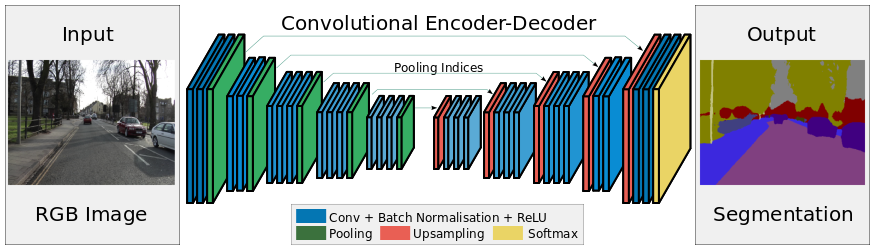
\includegraphics[width=0.75\linewidth]{literatuurstudie/segnet.png}
            \caption{Het SegNet~\cite{Badrinarayanan} segmentatie netwerk.}
            \label{fig:segnet_cnn}
        \end{figure}

        Het segmentatienetwerk SegNet~\cite{Badrinarayanan} is een combinatie van convolutielagen en pooling layers. Er zijn geen fully connected layers aanwezig zoals het geval is bij een classificatie netwerk.
        De bedoeling van het SegNet netwerk is om als output opnieuw een afbeelding te genereren. Hiervoor zijn de lagen opgebouwd als een zandloper. Op deze manier is de output even groot als de oorspronkelijke afbeelding.
        Een segmentatienetwerk wordt getraind op gelijkaardige manier aan een traditioneel \gls{cnn} met als verschil dat de labeling gebeurdt op pixelbasis aangezien de output even groot is als de input van het systeem.
        Het systeem geeft als output een label voor elke pixel uit de afbeelding onderverdeeld in de classen waarmee het systeem getraind is.

        Het SegNet netwerk is getraind op de SUN RGB-D~\cite{Song_2015_CVPR} dataset. Deze dataset bevat een groot aantal indoor scenes, waarbij er onder andere segmentatie klassen zijn voor muren, vloeren en plafonds.
        De training is gebeurd met enkel de \gls{rgb} gegevens van de dataset.
        Deze segmentatietechniek zou nuttig kunnen zijn voor dit onderzoek om in beelden bijvoorbeeld de vloer te kunnen onderscheiden.
